\chapter{Groundwater flow -- H-Processes}
\label{sec:Groundwater}
%
This chapter deals with saturated subsurface flow. In the aquifer concept balance equations determine strictly horizontal flow and vertical flow can be included by leakage terms through confining beds. The leakage terms add or subtract water from aquifers overlying and underlying a leaky confining bed according to the aquifer's head difference and a confining bed conductivity. An aquifer which contains a water table is termed unconfined and a completely filled aquifer is termed confined. The governing equations for three-dimensional groundwater, confined, and unconfined aquifer flow are introduced in Sec.~\ref{sec:Groundwater_theory}.
In Sec.~\ref{sec:Groundwater_confined} the benchmarks for confined and in Sec.~\ref{sec:Groundwater_unconfined} for unconfined aquifers are introduced. Groundwater flow is solved two- and three dimensionally in the benchmark examples.

\section{Theory}
\label{sec:Groundwater_theory}
%
A three-dimensional description of groundwater flow is given by the mass balance equation
%
\begin{eqnarray}
S_s\frac{\partial h}{\partial t}
- \nabla\cdot \frac{\rho g}{\mu} {\kappa} \nabla h
= q^{ex}
\label{eqn:GW_Governing}
\end{eqnarray}
%
where the head $h$ is the primary variable of groundwater flow and $S_s$ is the specific storage which is assumed to be independent of the head neglecting fluid and soil matrix compression. Use of Darcy's law for momentum balance leads to the fluid density $\rho$, dynamic fluid viscosity $\mu$, gravity constant $g$, and aquifer permeability matrix ${\kappa}$. Finally $q^{ex}$ denotes external sources and sinks.
Depth integration leads to the two-dimensional Boussinesq equation which describes unconfined aquifers and reads
%
\begin{eqnarray}
S_y\frac{\partial h}{\partial t}
- \nabla\cdot \frac{\rho g h}{\mu}  {\kappa}  \nabla h
= q^{ex}
\label{eqn:GW_unconfinedGoverning}
\end{eqnarray}
%
where $S_y$ is the specific yield.
For confined aquifers Eq.~\ref{eqn:GW_unconfinedGoverning} becomes
%
\begin{eqnarray}
S\frac{\partial h}{\partial t}
- \nabla\cdot \frac{\rho g L}{\mu}  {\kappa}  \nabla h
 = q^{ex}
\label{eqn:GW_confinedGoverning}
\end{eqnarray}
%
where $S$ is the storage and $L$ the aquifer thickness.
The aquifer thickness $L$ is taken into account by changing the soil permeability ${\kappa }$ in the following benchmark examples.
A channel source term can be assigned according to
%
\begin{eqnarray}
q^{ex} = K_{\Lambda} \frac{P}{B}\frac{h^{sur} - h^{sub}}{a}
\label{eqn:GW_riverSource}
\end{eqnarray}
%
where $K_{\Lambda}$ is the channel bed conductivity, $B$ the channel width, $a$ the channel bed thickness, and $h^{sur}$ the channel flow head. The wetted perimeter $P= 2 (h^{sur}-z^{sur}) + B$ for rectangular channel where $z^{sur}$ is the height of the top of the channel bed. Groundwater head $h$ is taken into account by
%
\begin{eqnarray}
h^{sub} = \max\left( h, z^{sur}\right).
\end{eqnarray}
%
Leakage terms between adjacent aquifers can be defined accordingly.
%
%--------------------------------------------------------------------------------------------------------------------------
\section{Linear groundwater flow}


\textbf{Theory}

Water flow in a saturated porous medium is influenced by the pressure gradient over a given distance and the hydraulic conductivity of the aquifer. By Darcy's Law (equ. \ref{eq21}) the flow rate by considering these influences can be calculated.
\begin{equation}
v_f\,=\,k_f\cdot i
\label{eq21}
\end{equation}
{\small
with
\begin{itemize}
\item[$v_f$] -- flow rate (m/s),
\item[$k_f$] -- hydraulic conductivity (m/s),
\item[$i$] -- pressure gradient (-).
\end{itemize}
}

The hydraulic conductivity is calculated by the following relation.
\begin{equation}
k_f\,=\,\frac{\kappa\cdot\rho\cdot g}{\mu}
\label{eq22}
\end{equation}
{\small
with
\begin{itemize}
\item[$\kappa$] -- permeability (m$^2$)
\item[$\rho$] -- density of the fluid (kg$\cdot$m$^{-3}$)
\item[$g$] -- gravity constant (m$\cdot$s$^{-2}$)
\item[$\mu$] -- dynamic viscosity of the fluid (Pa$\cdot$s)
\end{itemize}
}

By using the law of continuity the discharge through a defined cross section can be calculated.
\begin{equation}
Q\,=\,v_f\cdot A
\label{eq23}
\end{equation}
{\small
with
\begin{itemize}
\item[$Q$] -- discharge (m$^3$/s)
\item[$A$] -- cross section (m$^2$)
\end{itemize}
}

Layered soil material is possibly less permeable in one direction than in the direction perpendicular to it. In this case the input of different values for the permeability $\kappa$ in dependence on the direction of anisotropy is possible in RockFlow.


\subsection{Flow in an isotropic medium}


\subsubsection*{Problem definition}

This test example for groundwater flow is taken from the RockFlow Tutorial A (Ma{\ss}mann, 2004). The aim of this example is to simulate the stationary groundwater flow in a homogeneous aquifer. Figure \ref{fig21} shows a sketch of the calculation area.
\begin{figure}[htbp]
\centering
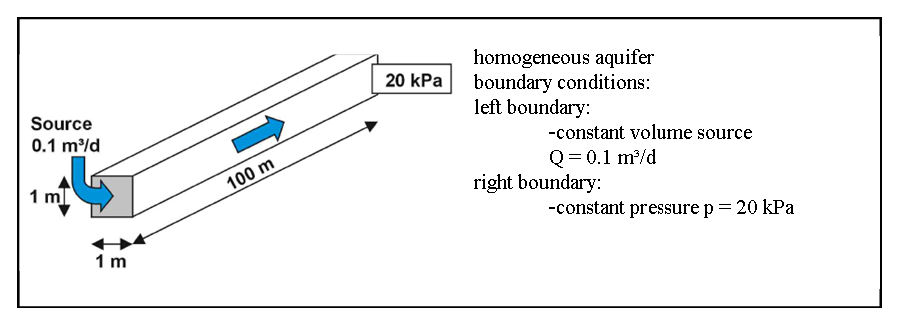
\includegraphics[width=1.0\textwidth]{H_GW/figures/fig21.eps}
\caption{Calculation area: homogeneous aquifer (Ma{\ss}mann, 2004)}
\label{fig21}
\end{figure}

\textsl{Assumptions}

\begin{tabbing}
\=xxxxxxxxxxxxx  \=xxxxxxxxxxxxxxxxxxxxxxx \kill
\> Aquifer: \> homogeneous, saturated, stationary flow
\end{tabbing}

\subsubsection*{Model set-up of the 1~D numerical model}

For the 1-dimensional calculation the calculation area is simplified as a line of a length of 100~m. The calculation model includes 100 elements and 101 nodes. As boundary condition the source volume of the fluid phase of 0.1~m$^3$/d is given at the left border of the calculation area and the constant pressure of 20~kPa at the right boundary. The used parameters of the soil are listed in table \ref{tab21}.
\begin{table}[htbp]
\centering
\begin{tabular}{|c|l|l|}
\hline
parameter & value & unit \\
\hline
porosity $\Phi$  & 0.2 &  --  \\			
\hline
permeability $\kappa$ & 1.0$\cdot 10^{-12}$ & m$^2$ \\
\hline
\end{tabular}
\caption{Used parameters}
\label{tab21}
\end{table}

\subsubsection*{Evaluation method}

The constant flow rate $v_f$ is calculated by using equation \ref{eq23}. In order to calculate the pressure at the left border of the calculation model, Darcy's Law is applied in the following way. The second relation (eq. \ref{eq24}) shows that the pressure gradient is linear.
\begin{equation}
i\,=\,\frac{Q}{k_f\cdot A}\,=\,
\frac{Q}{K\cdot\frac{\displaystyle{\rho\cdot g}}{\displaystyle{\eta}}\cdot A}\,=\,
\frac{1.157\cdot 10^{-6}\,\frac{\displaystyle{\mathrm{m}^3}}{\displaystyle{\mathrm{s}}}}
{9.81\cdot 10^{-6}\,\frac{\displaystyle{\mathrm{m}}}{\displaystyle{\mathrm{s}}}\cdot 1\,\mathrm{m}^2}
\quad\mathrm{and}\quad
p_{\mathrm{left}}\,=\,p_{\mathrm{right}}\,+\,\rho\cdot g\cdot i\cdot l
\label{eq24}
\end{equation}

\begin{figure}[htbp]
\centering
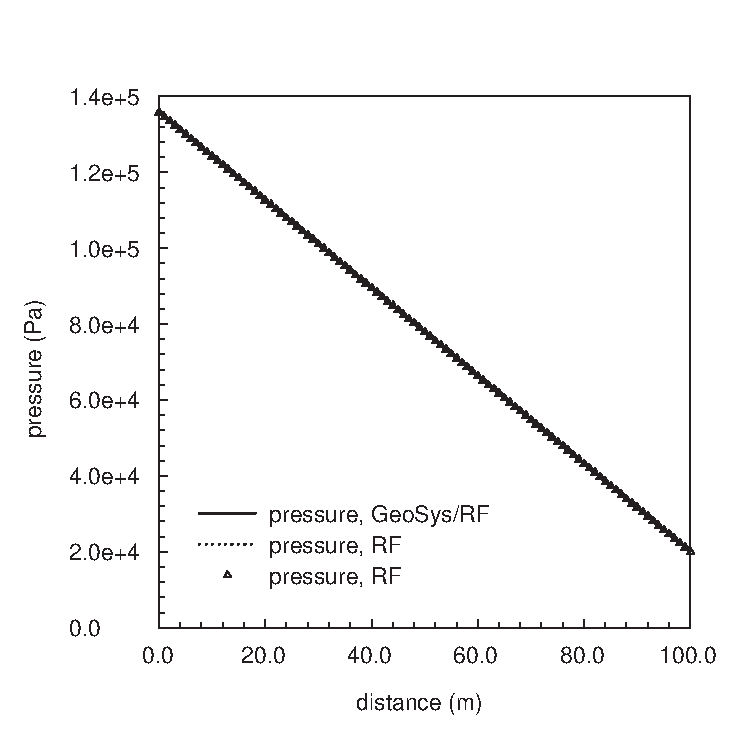
\includegraphics[width=0.5\textwidth]{H_GW/figures/fig22.eps}
\caption{Pressure distribution over the distance of 100~m}
\label{fig22}
\end{figure}

\subsubsection*{Results}

In figure \ref{fig22} you can find the pressure distribution over the whole length of the 1~D model that was calculated by GeoSys/RockFlow. In addition, the analytically calculated pressure distribution is depicted in this figure. These pressure values match the numerical results well.

\begin{tabular}{|l|l|l|}
\hline
Benchmark & Problem type	& Path in benchmark deposit \\
\hline	
h\_sat\_flow\_1d	& H	& benchmarks $\backslash$H$\backslash$sat\_1D \\
\hline	
\end{tabular}


\subsection{Flow in an anisotropic medium}


\subsubsection*{Problem definition}

The aim of this example is to simulate the stationary groundwater flow in an anisotropic porous medium. In order to consider the anisotropy of permeability, a 2~D numerical model was built which contains a higher permeability in the vertical than in the horizontal direction.

\textsl{Assumptions}

\begin{tabbing}
\=xxxxxxxxxxxxx  \=xxxxxxxxxxxxxxxxxxxxxxx \kill
\> Aquifer: \> anisotropic, saturated, stationary flow
\end{tabbing}

\subsubsection*{Model set-up of the 2~D numerical model}

For the 2-dimensional simulation, the cube consisting of a porous medium is simplified as a square with an area of 1~m$^2$. The calculation model includes 736 triangular elements and 409 nodes. At the left corner at the bottom of the model a constant pressure of 1000~Pa is specified along two polylines of the length of 0.3~m (\ref{fig23}). At the top and the right border the pressure is set to 0 in order to create a pressure gradient. As the porous medium is assumed to be anisotropic, which influences the groundwater flow, the values for permeability are equal to 1.0$\cdot 10^{-15}$ m$^2$ in x-direction and 1.0$\cdot 10^{-14}$ m$^2$ in y-direction.

\begin{table}[htbp]
\centering
\begin{tabular}{|c|l|l|}
\hline
parameter & value & unit \\
\hline
porosity $\Phi$  & 0.2 &  --  \\			
\hline
permeability $\kappa_x$ & 1.0$\cdot 10^{-15}$ & m$^2$ \\
\hline
permeability $\kappa_y$ & 1.0$\cdot 10^{-14}$ & m$^2$ \\
\hline
\end{tabular}
\caption{Used parameters}
\label{tab22}
\end{table}

\begin{figure}[htbp]
\centering
\includegraphics[width=1.0\textwidth]{H_GW/figures/fig23.eps}
\caption{Calculation model (2~D)}
\label{fig23}
\end{figure}

\subsubsection*{Evaluation method}
This test example is not made up to introduce a new process, but it shows the possibility for the GeoSys/RockFlow user to give a specific permeability for each direction. Therefore, the interpretation of GeoSys/RockFlow results comprises merely the comparison between pressure distributions due to anisotropic groundwater flow that were simulated by the use of RockFlow and GeoSys/RockFlow. This comparison is possible because both versions are developed separately concerning anisotropy of soils.

\begin{figure}[htbp]
\centering
\includegraphics[width=0.6\textwidth]{H_GW/figures/fig24.eps}
\caption{Pressure distribution caused by anisotropic saturated flow}
\label{fig24}
\end{figure}

\subsubsection*{Results}

In figure \ref{fig24} the horizontal and vertical pressure distributions of an anisotropic groundwater model which is made using the program code RockFlow are depicted next to the pressure distributions of the described anisotropic model. While presuming an anisotropic medium, an inhomogeneous pressure field is developing, because the groundwater is not able to spread out uniformly. This can be recognized at the different curve gradients in x- and y-direction. There are slight differences between the curve characteristics of the RockFlow and the GeoSys/RockFlow simulation results. These differences are due to different element types (square in the RockFlow model) and the resulting differing x- or y-coordinates. Therefore, the pressure distributions that are obtained by the simulation with GeoSys/RockFlow are evaluated to be correct.

\begin{tabular}{|l|l|l|}
\hline
Benchmark & Problem type	& Path in benchmark deposit \\
\hline	
H\_sat\_flow\_K\_ortho	& H	& benchmarks $\backslash$H$\backslash$sat\_2D \\
\hline	
\end{tabular}


\subsection{Flow in an isotropic and heterogeneous medium}


\subsubsection*{Problem definition}

The aim of this example is to simulate the stationary groundwater flow in an isotropic and heterogeneous porous medium. In order to consider the heterogeneous of permeability, a 2~D numerical model was built. The heterogeneous distribution of permeability is showed in \ref{KDis}.
\begin{figure}[htbp]
\centering
\includegraphics[width=0.8\textwidth]{H_GW/figures/KDis.eps}
\caption{Calculation model(2~D): hetergeneous permeability distribution}
\label{KDis}
\end{figure}

\textsl{Assumptions}

\begin{tabbing}
\=xxxxxxxxxxxxx  \=xxxxxxxxxxxxxxxxxxxxxxx \kill
\> Aquifer: \> isotropic, heterogeneous, saturated, stationary flow
\end{tabbing}

\subsubsection*{Model set-up of the 2~D numerical model}

For the 2-dimensional simulation, the cube consisting of a porous medium is simplified as a square with an area of 10000~m$^2$. The calculation model includes 10000 quad elements and 10201 nodes. At the left boundary  a constant head of 10~m and the right boundary  a constant head of 9~m are specified in order to create a pressure gradient. 

\subsubsection*{Results}

In figure \ref{HeadDis} the horizontal and vertical head distributions of a groundwater flow in a heterogeneous medium are depicted responsing to the distribution of the permeability. 

\begin{figure}[htbp]
\centering
\includegraphics[width=0.8\textwidth]{H_GW/figures/HeadDis.eps}
\caption{Head distribution responsed to isotropic and heterogeneous medium}
\label{HeadDis}
\end{figure}

\begin{tabular}{|l|l|l|}
\hline
Benchmark & Problem type	& Path in benchmark deposit \\
\hline	
2D1P-GWFlow	& H	& benchmarks $\backslash$H$\backslash$HetGWFlow \\
\hline	
\end{tabular}
%--------------------------------------------------------------------------------------------------------------------------
%
\section{Confined aquifer}
\label{sec:Groundwater_confined}
%
%--------------------------------------------------------------------------------------------------------------------------
\subsection{Constant source term}
\label{sec:Groundwater_confined_source}
%
\subsubsection*{Problem definition}
%
These examples deal with an aquifer which is subject to a constant recharge line source.
\cite{Glover:78} presented an analytical solution for a constant line source on an infinite domain which reads for the groundwater head at the source
%
\begin{eqnarray}
h = q^{ex}\sqrt{ \frac{\mu t}{\pi \rho g k L S_y}}. \label{GW_Glover}
\end{eqnarray}
%
The aquifer size is $20m\times 10m$ with the source term at one boundary (See Fig.~\ref{GW_riv1_domain}). The simulation time is $30min$.
%
\subsubsection*{Initial and boundary conditions}
%
Initial groundwater head is $0m$. The source term is $2\times 10^{-4} m/s$, groundwater head is $0$ at the opposite boundary, and at the remaining part no-flow is imposed.
\subsubsection*{Material properties}
%
For the spatial discretization $24\times 12$ quadrants or hexahedra are used. The hexahedra have a height of $1m$.
Material parameters are given in Tab.~\ref{GW_SourceTerm}.
%
\begin{table}[H]
 \centering
 \caption{Parameters for the constant source term examples}
 \centering \label{GW_SourceTerm}
 \begin{tabular}{llll}
 \hline\hline\noalign{\smallskip}
 {\bf Parameter} & {\bf Symbol} & {\bf Setting} & {\bf Unit} \\ \hline
 Storage & $S$ & $0.2$ & $-$ \\
 Specific storage & $S_s$ & $0.2$ & $1/m$ \\
 Viscosity  & $\mu$ & $1\times 10^{-3}$ & $Pa\cdot s$\\
 Thickness & $L$ & $1$ & $m$ \\
 \noalign{\smallskip}\hline\hline
 \end{tabular}
\end{table}
%
\subsubsection*{Results}
%
Simulation results are compared with the analytical solution in Fig.~\ref{GW_Results_Source}
%
\begin{figure} [htb!]
 \centering
\includegraphics[width=0.6\columnwidth] {H_GW/figures/q_hex_point.eps}
\caption{Results and analytical solution for confined aquifer with line source term}
 \label{GW_Results_Source}
\end{figure}
%
\subsubsection*{Benchmark deposit}
%
\begin{tabular}{|l|l|l|}
  \hline
  Benchmark & Problem type & Path in benchmark deposit \\
  \hline
  \emph{q\_quad} & H & benchmarks\verb \GROUNDWATER_FLOW\ \\
  \emph{q\_hex} & H & benchmarks\verb \GROUNDWATER_FLOW\ \\
  \hline
\end{tabular}
%
%--------------------------------------------------------------------------------------------------------------------------
%
\subsection{Channel source term}
\label{sec:Groundwater_confined_channelSource}
%
\subsubsection*{Problem definition}
%
For these examples the source term of the previous examples (Sec.~\ref{sec:Groundwater_confined_source}) is substituted by a corresponding channel source term (Eqn.~\ref{eqn:GW_riverSource}). The channel is assumed to be not affected by the water loss and the exchange flux is independent of the groundwater head. Therefore, the source term represents a steady and uniform channel located above the aquifer. The cross-section of the channel is rectangular. The setup, spatial discretization, and calculated water head are shown in Fig.~\ref{GW_riv1_domain}. The simulation time is $30min$.
%
\begin{figure} [htb!]
 \centering
\includegraphics[width=0.7\columnwidth] {H_GW/figures/q_hex.eps}
\vspace{-2cm}
\caption{Computational domain and (channel) source term location}
 \label{GW_riv1_domain}
\end{figure}

%
\subsubsection*{Initial and boundary conditions}
%
The initial groundwater head is $0m$. The channel source term is the boundary condition at one side, at the opposite boundary the head is fixed $0$. At the remaining boundaries no-flow is imposed.
\subsubsection*{Material properties}
%
For the spatial discretization either $24\times 12$ quadrants or hexahedra are used as well prisms which are generated by cutting the hexahedra in two parts. The hexahedra or prism height is $1m$. The time step is $1 min$.
Simulation parameters for the aquifer and the channel source term are given in Tab.~\ref{GW_ChannelPercolation}.
%
\begin{table}[H]
 \centering
 \caption{Parameters for channel source term examples}
 \centering \label{GW_ChannelPercolation}
 \begin{tabular}{llll}
 \hline\hline\noalign{\smallskip}
  {\bf Parameter} & {\bf Symbol} & {\bf Setting} & {\bf Unit} \\ \hline
 {\bf Aquifer} & & & \\
 Storage & $S$ & $0.2$ & $-$ \\
 Specific storage & $S_s$ & $0.2$ & $1/m$ \\
 Viscosity  & $\mu$ & $1\times 10^{-3}$ & $Pa\cdot s$\\
 Thickness & $L$ & $1$ & $m$ \\ \hline
 {\bf Channel source term} & & & \\
 Head & $h^{sur}$ & $4$ & $m$ \\
 Bed top location& $z^{sur}$ & $1$ & $m$ \\
 Width & $B$ & $14$ & $m$ \\
 Conductivity & $K_{\Lambda}$ & $1\times 10^{-6}$ & $m/s$ \\
 Thickness & $a$ & $0.3$ & $m$ \\
 \noalign{\smallskip}\hline\hline
 \end{tabular}
\end{table}
%
\subsubsection*{Results}
%
Comparison of simulation results and analytical solution is given in Fig.~\ref{GW_Results_ChannelPercolation_quad}
for quadrants and in Fig.~\ref{GW_Results_ChannelPercolation_hex} for hexahedra.
%
\begin{figure} [htb!]
 \centering
\includegraphics[width=0.6\columnwidth] {H_GW/figures/riv1_quad_point.eps}
\caption{Results with quadratic elements and analytical solution for confined aquifer below uniform and steady channel}
 \label{GW_Results_ChannelPercolation_quad}
\end{figure}
%
\begin{figure} [htb!]
 \centering
\includegraphics[width=0.6\columnwidth] {H_GW/figures/riv1_hex_point.eps}
\caption{Results with hexahedral and prismatic elements compared with the analytical solution for confined aquifer below uniform and steady channel}
 \label{GW_Results_ChannelPercolation_hex}
\end{figure}
%
\subsubsection*{Benchmark deposit}
%
\begin{tabular}{|l|l|l|}
  \hline
  Benchmark & Problem type & Path in benchmark deposit \\
  \hline
  \emph{riv1\_quad} & H & benchmarks\verb \GROUNDWATER_FLOW\ \\
  \emph{riv1\_pris} & H & benchmarks\verb \GROUNDWATER_FLOW\ \\
  \emph{riv1\_hex} & H & benchmarks\verb \GROUNDWATER_FLOW\ \\
 \hline
\end{tabular}
%
%--------------------------------------------------------------------------------------------------------------------------
%
\subsection{Channel sink term}
%
\subsubsection*{Problem definition}
%

For this example the channel of the previous examples (Sec.~\ref{sec:Groundwater_confined_channelSource}) is located such that flow from the aquifer to the channel takes place. Therefore, the source term represents a steady and uniform rectangular channel located in the aquifer. The setup is shown in Fig.~\ref{GW_riv1_domain}. The simulation time is $30min$.


\subsubsection*{Initial and boundary conditions}
%
Initial groundwater head is $0m$. The channel source term is the boundary condition at one side, at the opposite boundary the head is $0$. At the other boundaries no-flow is imposed.
\subsubsection*{Material properties}
%
The domain is discretization with $24\times 12$ quadrants. The time step size is $1 min$.
Simulation parameters for the aquifer and the channel source term are given in Tab.~\ref{GW_ChannelPercolation}.
%
\begin{table}[H]
 \centering
 \caption{Parameters for the channel sink term example}
 \centering \label{GW_ChannelPercolation}
 \begin{tabular}{llll}
 \hline\hline\noalign{\smallskip}
 {\bf Parameter} & {\bf Symbol} & {\bf Setting} & {\bf Unit} \\ \hline
 {\bf Aquifer} & & & \\
 Storage & $S$ & $0.2$ & $-$ \\
 Specific storage & $S_s$ & $0.2$ & $1/m$ \\
 Viscosity  & $\mu$ & $1\times 10^{-3}$ & $Pa\cdot s$\\
 Thickness & $L$ & $1$ & $m$ \\ \hline
 {\bf Channel source term} & & & \\
 Head & $h^{sur}$ & $-0.5$ & $m$ \\
 Bed top location& $z^{sur}$ & $-0.7$ & $m$ \\
 Width & $B$ & $59.6$ & $m$ \\
 Bed conductivity & $K_{\Lambda}$ & $1\times 10^{-6}$ & $m/s$ \\
 Bed thickness & $a$ & $0.3$ & $m$ \\
 \noalign{\smallskip}\hline\hline
 \end{tabular}
\end{table}
%
\subsubsection*{Results}
%
Simulation results are shown in Fig.~\ref{GW_Results_ChannelSink}.
%
\begin{figure} [htb!]
 \centering
\includegraphics[width=0.6\columnwidth] {H_GW/figures/riv2_hex_point.eps}
\caption{Results by GeoSys for confined aquifer with a constant channel sink term}
 \label{GW_Results_ChannelSink}
\end{figure}
%
\subsubsection*{Benchmark deposit}
%
\begin{tabular}{|l|l|l|}
  \hline
  Benchmark & Problem type & Path in benchmark deposit \\
  \hline
  \emph{riv2\_hex} & H & benchmarks\verb \GROUNDWATER_FLOW\ \\
  \hline
\end{tabular}
%
%--------------------------------------------------------------------------------------------------------------------------
%
\subsection{Theis' Problem}
%
\subsubsection*{Problem definition}
%
Theis' problem examines the transient lowering of the water table induced by a pumping well. Theis' fundamental insight was to recognize that Darcy's law is analogous to the law of the flow of heat by conduction, hydraulic pressure being analogous to temperature, pressure-gradient to thermal gradient.
%
\subsubsection*{Assumptions}
%
\textit{Aquifer:} confined, infinite areal extend, homogeneous, isotropic, uniform thickness, horizontal piezometric surface;\\
\textit{Well:} constant discharge rate, well penetrates the entire thickness, well storage effects can be neglected.\\
%
\subsubsection*{Analytical solution}
The analytical solution of the drawdown as a function of time and distance is expressed by equation ~\ref{theis}:
%
\begin{eqnarray}
h_0 - h(t,x,y) = \frac{Q}{4\pi T}W(u)
\label{theis}
\end{eqnarray}
%
\begin{eqnarray}
u = \frac{(x^{2}+y^{2})S}{4Tt}
\label{theis_u}
\end{eqnarray}
%
where:\\ \\
%
\begin{tabular}{|l|l|l|}
  \hline
  symbol & property & unit \\
  \hline
  \ $h_0$ & constant initial hydraulic head & L \\
  \hline
  \ Q & constant discharge rate & $L^{3}T^{-1}$ \\
  \hline
  \ T & aquifer transmissivity & $L^{2}T^{-1}$\\
  \hline
  \ t & time & T\\
  \hline
  \ x,y & the coordinate at any point & L\\
  \hline
  \ S & aquifer storage & -\\
  \hline
\end{tabular}
%

\subsubsection*{Initial and boundary conditions}
%
\begin{tabular}{|l|l|}
  \hline
  Parameters/conditions & OpenGeoSys \\
  \hline
  Initial conditions & h(0,r)=0  \\
  \hline
  Sink, well pumping rate & $Q=1.22329\times 10^{3} m^{3} d^{-1}$  \\
  \hline
  Boundary conditions & h(t,304.8m)=0  \\
  \hline
   flow materials&   \\
  \hline
    -Hydraulic conductivity & $9.2903\times 10^{-4}m s^{-1}$  \\
  \hline
    -storage coefficient & S=0.001   \\
  \hline
    -storage compressibility & 0  \\
  \hline
    -wellbore radius & 0.3048m  \\
  \hline
\end{tabular}
%
\begin{figure} [htb!]
 \centering
\includegraphics[width=0.7\columnwidth] {H_GW/figures/Theis1.eps}
\caption{Calculated drawdowns at a distance of 9.639m from the well.}
 \label{Theis1}
\end{figure}
%
%
\subsubsection*{Results}
Fig.~\ref{Theis1} shows the comparison of analytically and numerically caculated drawdown of hydraulic head versus time at the distance of r = 9.639 m from the well.
\subsubsection*{Benchmark deposit}
%
\begin{tabular}{|l|l|l|}
  \hline
  Benchmark & Problem type & Path in benchmark deposit \\
  \hline
  \emph{h\_quad\_axisym} & H & benchmarks\verb \H\Theis_1D\ \\
  \hline
\end{tabular}

%
\begin{figure} [htb!]
 \centering
 \includegraphics[width=0.9\columnwidth] {H_GW/figures/theis2.eps}
 \caption{Cone of depression at the end of the simulation.}
 \label{theis2}
\end{figure}
%
%
\subsubsection*{2D application}
%
The 2D application is solved in the following situation:\\
\\
%
\begin{tabular}{|l|l|l||l|}
  \hline
  parameters& description & values & unit \\
  \hline
  Q & discharge rate & 1000  & $m^{3}d^{-1}$  \\
  S & specific storage & $1.0\times 10^{-5}$ & $m^{-1}$ \\
  T & transmissivity & 1000 &  $m^{2}d^{-1}$ \\
  B & thickness of aquifer & 20 & m \\
  \hline
\end{tabular}
\\
\\
The aquifer horizontal domain size is 1000m $\times$ 750 m with the pumping well at the location coordinate (500,375).The discretization of space is 10m $\times$ 10m grid. The simulation time is 0.00175 day and the time step is 1.036 sec. The boundary condition is 0.0 drawdown.
The cone of depression induced by the pumping well at the end of the simulation is plotted in Fig.~\ref{theis2}.
\subsubsection*{Benchmark deposit}
%
\begin{tabular}{|l|l|l|}
  \hline
  Benchmark & Problem type & Path in benchmark deposit \\
  \hline
  \emph{h\_quad\_axisym} & H & benchmarks\verb \H\Theis_2D\ \\
  \hline
\end{tabular}
%

%----------------------------------------------------------------------------------------------------------------------------------

\section{Time variant flow}

This benchmark is set up to test the implementation of time variant boundary conditions for the \texttt{GROUNDWATER\_FLOW} process. These boundary conditions allow to simulate flow and transport in a flow field, which changes gradient and direction according to user specified functions.

The setup of the model domain is depicted in Figure \ref{time_variant_flow_setup}. The model geometry is designed by 4 corner nodes (gli nodes 0 through 3), which are connected along the model edges by one polyline each. To induce a time variant flow field, time functions are generated externally and are connected to the corner gli nodes. The polyline names and location and the names of the time functions are shown in Figure \ref{time_variant_flow_setup}.

To connect the time functions with the boundary condition, the boundary condition has to be specified along a polyline. The distribution type is \texttt{LINEAR} followed by the number of nodes of the polyline (2) and then by two lines specifying the gli node number, the value at this node and the name of the time function. The value of the time function at the corresponding time is then multiplied by the specified value at the nodes and interpolated to all mesh nodes found along the polyline. This is performed in each timestep. In the case shown here, this was applied for all four boundary condition polylines along the four model area sides.

\small
\begin{verbatim}
#BOUNDARY_CONDITION
 $PCS_TYPE
  GROUNDWATER_FLOW
 $PRIMARY_VARIABLE
  HEAD
 $GEO_TYPE
  POLYLINE BCLEFT
 $DIS_TYPE
  LINEAR 2
   0 1.0 BC_left_low
   3 1.0 BC_left_high
   \end{verbatim}
\normalsize

The model area is 184 m in x direction and 64 m in y direction. Boundary conditions are placed along all four sides of the model area. Hydraulic conductivity is 0.00215 m s$^{-1}$, the storage coefficient is set to 0. Initial conditions are a head of 2.0239 m everywhere.

The benchmark tests at the same time the application of a heterogeneous distribution of the hydraulic conductivity. This is achieved by setting in the *.mmp file:
\small
\begin{verbatim}
 $PERMEABILITY_TENSOR
  ISOTROPIC 1.0
 $PERMEABILITY_DISTRIBUTION
  2d_het_a_kfhet
\end{verbatim}
\normalsize

The file \texttt{2d\_het\_a\_kfhet} contains the heterogeneous distribution of the hydraulic conductivity, and is generated using an geostatistical simulator. The file contains information on the \texttt{\$MSH\_TYPE}, the \texttt{\$MMP\_TYPE} and specifies options for the interpolation of the values onto the elements of the specified mesh (\texttt{\$DIS\_TYPE}). Under the keyword \texttt{\$DATA} the actual values are specified as x - y - parameter values, where parameter is the hydraulic conductivity. The end of the data set is marked using the keyword \texttt{\#STOP}.

\small
\begin{verbatim}
#MEDIUM_PROPERTIES_DISTRIBUTED	
; Specify mesh, for which data is read
$MSH_TYPE
  GROUNDWATER_FLOW
$MMP_TYPE
 PERMEABILITY
; give interpolation option: NEAREST_VALUE or GEOMETRIC_MEAN
$DIS_TYPE
 NEAREST_VALUE
$CONVERSION_FACTOR
 1.0
; X, Y, Z, nof field values			
$DATA
33.00  35.00 0 1.0903602235e-004
25.00  37.00 0 8.4356781197e-005
125.00  21.00 0 5.7274327695e-005
...
\end{verbatim}
\normalsize




The result of the simulation is shown in Figures \ref{time_variant_heads_results} in top view. The full contours show the piezometric head isolines after the first five time steps, the black and red lines show head isolines from a succession of time steps. It can be seen, that the flow field is turned and directed upwards (black isolines) and back again (red isolines) during the simulation. Figure \ref{time_variant_heads_observationwell} shows the time variant head in an observation well at x=20 m and y=28 m. The rise and fall of the piezometric head due to the time variant flow field can be clearly seen, as well as the initial jump from the initial head to the time variant head.

\begin{figure}[htbp]
\centering
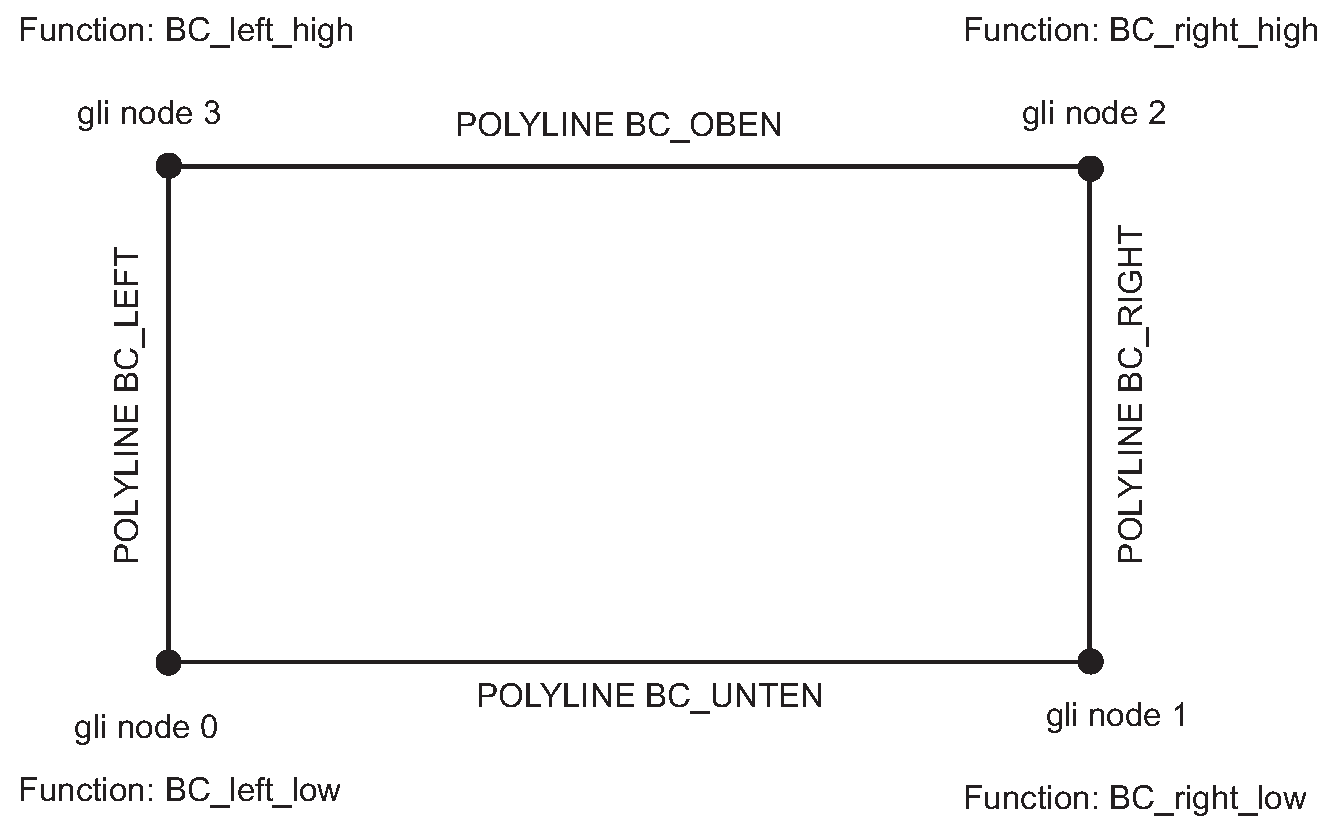
\includegraphics[width=0.6\textwidth]{H_GW/figures/time_variant_flow_setup.eps}
\caption{Model setup for the time variant flow}
\label{time_variant_flow_setup}
\end{figure}

\begin{figure}[htbp]
\centering
\includegraphics[width=0.75\textwidth]{H_GW/figures/time_variant_heads_results.eps}
\caption{Model results for the time variant heads in top view}
\label{time_variant_heads_results}
\end{figure}

\begin{figure}[htbp]
\centering
\includegraphics[width=0.4\textwidth]{H_GW/figures/time_variant_heads_observationwell.eps}
\caption{Model results at one observation well}
\label{time_variant_heads_observationwell}
\end{figure}

\begin{table}[htbp]
\centering
\begin{tabular}{|l|l|l|}
\hline
Benchmark & Type & Path \\
\hline
\texttt{transient\_flow}& H &  benchmarks$\backslash$GROUNDWATER\_FLOW$\backslash$transient\_flow  \\			
\hline
\end{tabular}
\end{table}


%--------------------------------------------------------------------------------------------------------------------------
%
\section{Unconfined aquifer}
\label{sec:Groundwater_unconfined}
%
\subsection{Steady state case}
%
\subsubsection*{Problem definition}
%
In these examples the aquifer consists of a small strip with the size of $100m \times 2m$ (see Fig.~\ref{GW_Results_uc}). At both ends the head is fixed and constant recharge is imposed on the whole domain which leads to steady state flow. This setting allows comparison with an analytical solution.
%\emph{uc\_quad}, \emph{uc\_tri} solve the two-dimensional Eqn.~\ref{eqn:GW_unconfinedGoverning}  for unconfined auifer and \emph{uc\_pris} solves the three-dimensional groundwater Eqn.\ref{eqn:GW_Governing}.
%
\subsubsection*{Initial and boundary conditions}
%
Initial groundwater head is $0m$. At one end of the strip the head is $1$ at the other $5$. At the top a source term of $1.0\times 10^{-8} m/s$ and at the remaining parts no-flow is imposed.
\subsubsection*{Material properties}
%
For the spatial discretization $100$ equal quadrants and $410$ triangles or prisms are used. In latter case the three-dimensional groundwater Eqn.~\ref{eqn:GW_unconfinedGoverning} is solved with elements adapting to the water height. One time step with the size of $100 s$ is used. The specific storage $S_s = 0 m^{-1}$ or specific yield $S_y = 0$ and a permeability $\kappa$ of $1\times 10^{-9} m^2$ is used.
%
\subsubsection*{Results}
%
Comparison of simulation results for prisms and analytical solution is shown in Fig.~\ref{GW_Results_uc}.
%
\begin{figure} [htb!]
 \centering
\includegraphics[width=0.7\columnwidth] {H_GW/figures/uc_pris.eps}
\caption{Results of unconfined aquifer benchmark example by GeoSys with prisms}
 \label{GW_Results_uc}
\end{figure}
%
\subsubsection*{Benchmark deposit}
%
\begin{tabular}{|l|l|l|}
  \hline
  Benchmark & Problem type & Path in benchmark deposit \\
  \hline
  \emph{uc\_quad} & H & benchmarks\verb \GROUNDWATER_FLOW\ \\
  \emph{uc\_tri} & H & benchmarks\verb \GROUNDWATER_FLOW\ \\
  \emph{uc\_pris} & H & benchmarks\verb \GROUNDWATER_FLOW\ \\
  \hline
\end{tabular}

%
%--------------------------------------------------------------------------------------------------------------------------
% 